% !TEX root = ../EjsS Manual.tex

\chapter{Exploring the Java flavor of \Ejs}\label{chapter:JavaEJS}

\begin{quote}
A good example is the best sermon.  {\em Benjamin Franklin}
\end{quote}

To  provide a perspective of the modeling process, in this chapter we first load, inspect, and run an existing simple harmonic oscillator simulation. We then modify the simulation to show how \ejs\ engages the user in the modeling process and greatly reduces the amount of
programming that is required. This chapter uses Java as the programming language for the modeling and is a twin chapter of Chapter~\ref{chapter:JavascriptEJS} (where Javascript is used).

% ------------------------
    \section{Inspecting the Simulation}\label{section:02ExplorationJavaInspecting}\index{\Ejs!inspecting a simulation}
% ------------------------

As mentioned in Chapter~\ref{chapter:EjsIntro}, \Ejs\ provides three workpanels for modeling. The first panel, \lit{Description}, allows us to create and edit multimedia HTML-based narrative that describes the model.\index{HTML} 
The second work panel, \lit{Model}, is dedicated to the modeling process. We use this panel to create
variables that describe the model, to initialize these variables, and to write algorithms that describe how this model
changes in time. The third workpanel, \lit{View}, is dedicated to the task of building the graphical user interface,
which allows users to control the simulation and to display its output.  

To understand how the \lit{Description}, \lit{Model}, and \lit{View} workpanels work together, we inspect and run an
already existing simulation. Screen shots are no substitute for a live demonstration, and you are encouraged to follow along on your computer as you read.

\begin{figure}[htb]
  \centering
  \subfigure{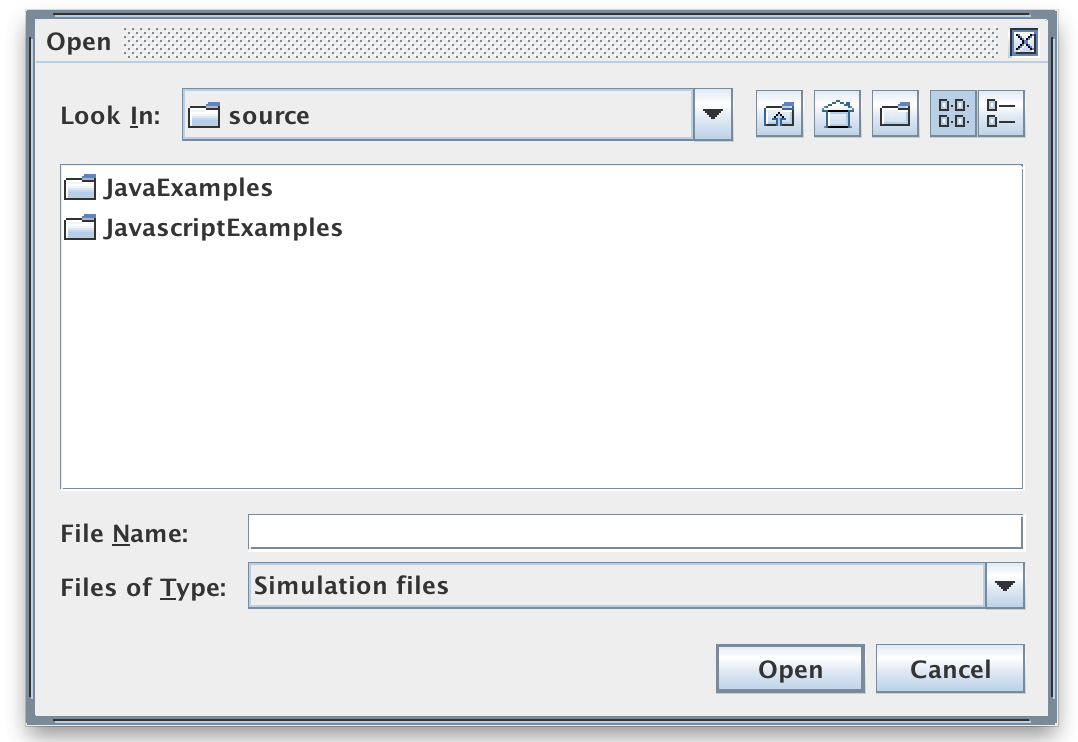
\includegraphics[scale=0.2]{02ExplorationJava/images/OpenDialogCrossPlatform.png}}
  \subfigure{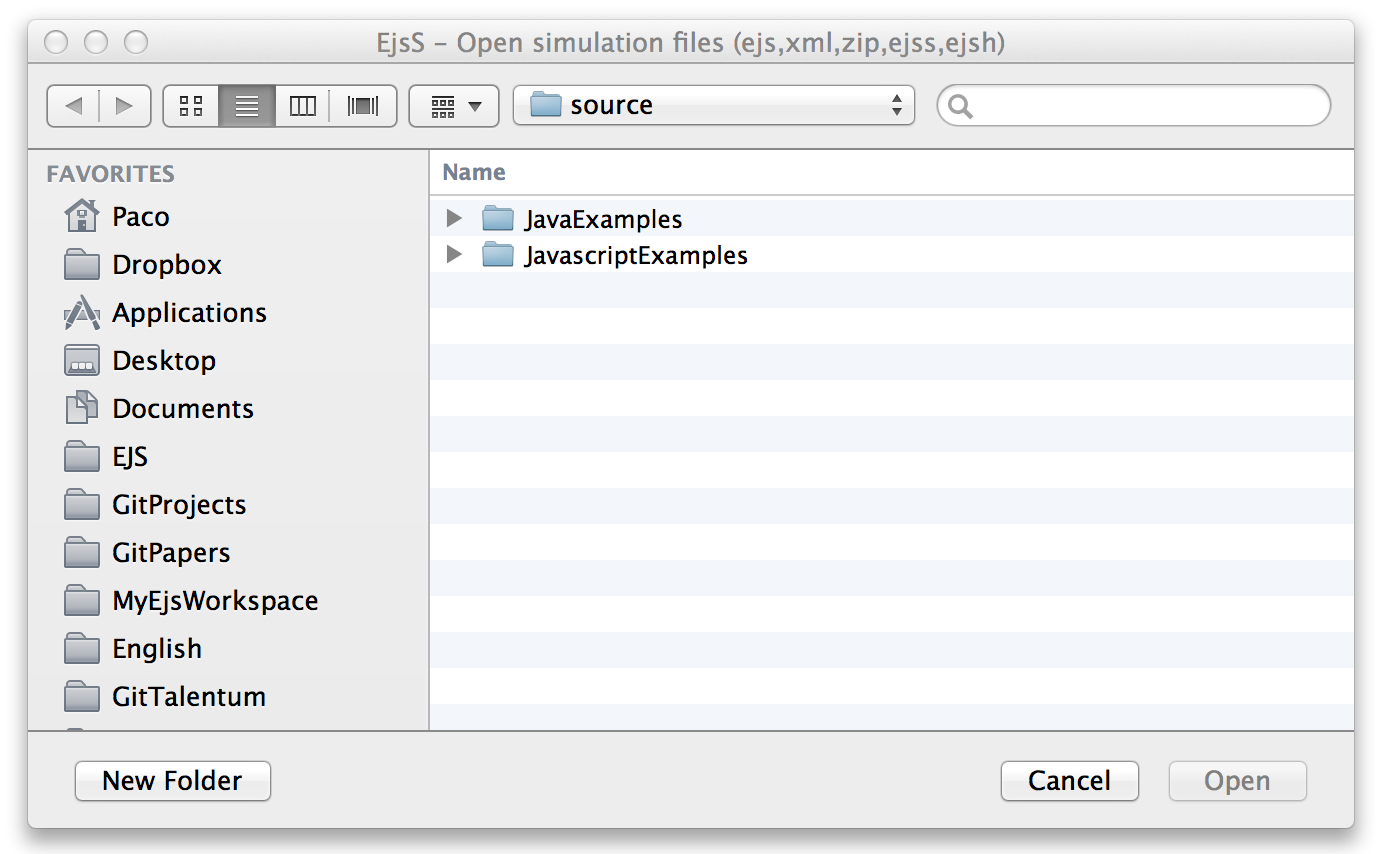
\includegraphics[scale=0.2]{02ExplorationJava/images/OpenDialogNative.png}}  
  \caption{The open file dialog lets you browse your hard disk and load an existing simulation. The appearance of the dialog 
  (shown here using two different look and feels) may vary, depending on your operating system and the selected \lit{look and feel}.}
  \label{fig:02ExplorationJava/OpenDialog}
\end{figure}

Click on the \lit{Open} icon 
\includegraphics[scale=\linescale]{../_common/icons_png/openSmall.png} on the \ejs\ taskbar. A file dialog
similar to that in Figure~\ref{fig:02ExplorationJava/OpenDialog} appears showing the contents of your workspace's \file{source}
directory. Go to the \file{JavaExamples} directory, where you will find a
file called \file{MassAndSpring.ejs}. Select this file and click on the \lit{Open} button of the
file dialog.

Now, things come to life! \ejs\ reads the \file{MassAndSpring.ejs} document which populates the workpanels and two new
``Ejs windows'' appear in your display as shown in Figure~\ref{fig:02ExplorationJava/SpringInterface}. A quick warning. You
can drag objects within these mock-up windows but this will set the model's initial conditions.  It is usually better
to set initial conditions using a table of variables as described in Section~\ref{section:02ExplorationJavaModel}.

\begin{figure}[htb]
  \centering
  \subfigure{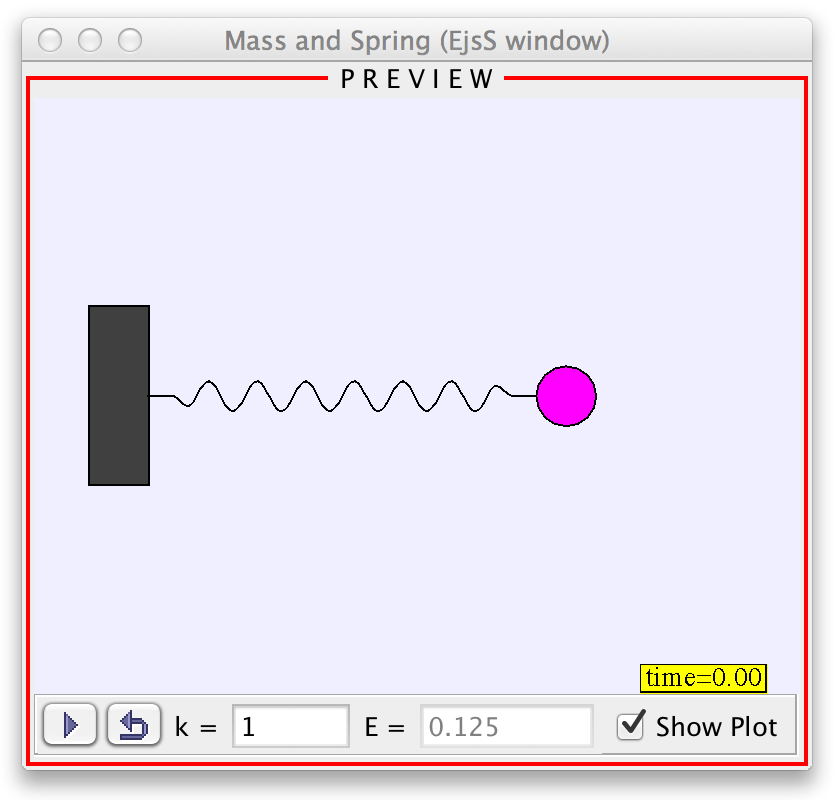
\includegraphics[scale=\scale]{02ExplorationJava/images/SpringInterface1.png}}
  \subfigure{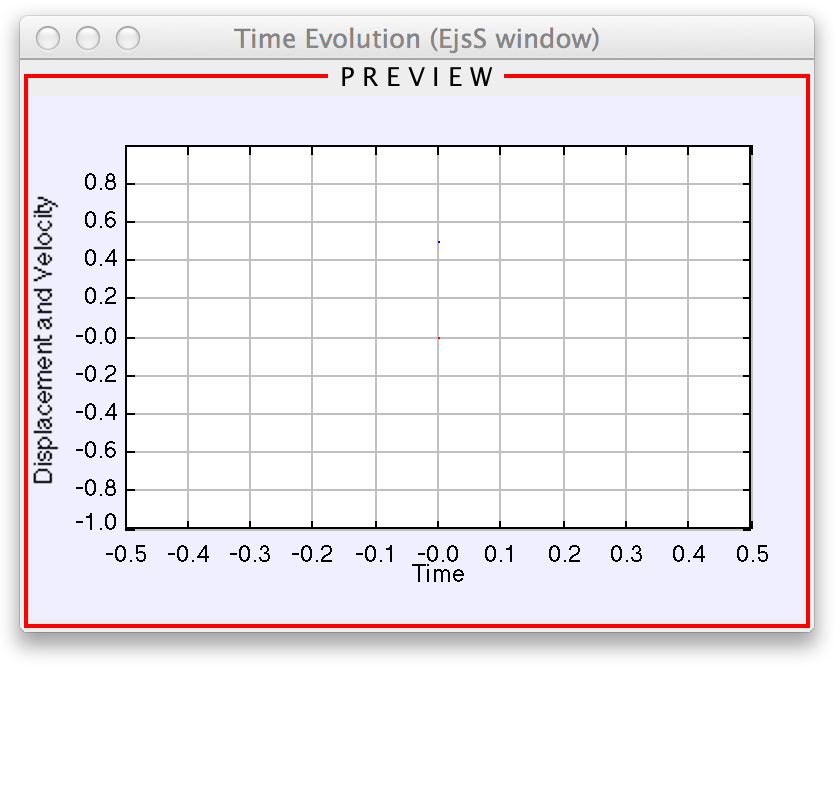
\includegraphics[scale=\scale]{02ExplorationJava/images/SpringInterface2.png}}
  \caption{\ejs\ mock-up windows of the \file{MassAndSpring} simulation. The title bar and the red border show that they are \ejs' windows
  and that the program is not running.}
  \label{fig:02ExplorationJava/SpringInterface}
\end{figure}

\note{Impatient or precocious readers may be tempted to click on the green run icon 
\includegraphics[scale=\linescale]{../_common/icons_png/launch.png} on the taskbar to execute our
example before proceeding with this tutorial.  Readers who do so will no longer be interacting with \ejs\  but with a compiled and running Java program.  Exit the running program by closing the \lit{Mass and Spring} window or by right clicking on the (now) red-squared stop icon 
\includegraphics[scale=\linescale]{../_common/icons_png/stop.png} on \ejs' taskbar before proceeding.}

\subsection{The \lit{Description} workpanel}

Select the \lit{Description}\index{Ejs!Description} workpanel by clicking on the corresponding radio button at the top of
\ejs, and you will see two pages of narrative for this simulation. The first page, shown in
Figure~\ref{fig:02ExplorationJava/SpringDesc}, contains a short discussion of the mass and spring model. Click on the
\lit{Activities} tab to view the second page of narrative.

\begin{figure}[htb]
  \centering
  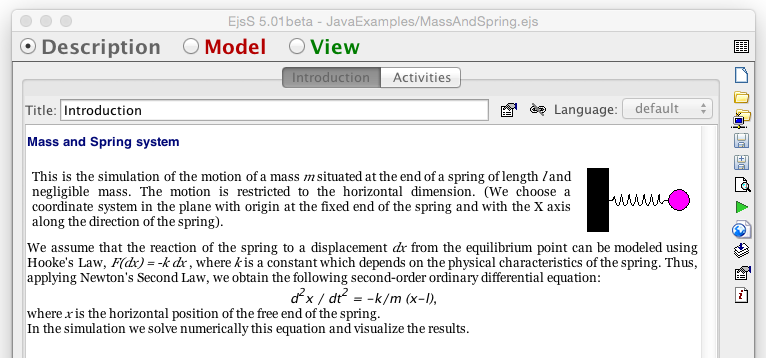
\includegraphics[scale=\scale]{02ExplorationJava/images/SpringDesc.png}
  \caption{The description pages for the mass and spring simulation. Click on a tab to display the page. Right-click on a tab to edit the page.}
  \label{fig:02ExplorationJava/SpringDesc}
\end{figure}

A \lit{Description} is HTML\index{HTML} or XHTML\index{XHTML} multimedia text that provides information and instructions about the
simulation. HTML stands for HyperText Markup Language and is the most commonly used protocol for formatting and
displaying documents on the Web. The X in XHTML stands for eXtensible. XHTML is basically HTML expressed as valid XML or, in simpler words, perfectly formatted HTML.

\ejs\ provides a simple HTML editor that lets you create and modify pages within \ejs.
You can also import HTML or (preferably) XHTML pages into \ejs\ by right clicking on a tab in the \lit{Description} workpanel. (See
Section~\ref{section:02ExplorationJavaModifyingDescription}.) Description pages are an essential part of the modeling process and
these pages are included with the compiled model when the model is exported for distribution.

\subsection{The \lit{Model} workpanel}\label{section:02ExplorationJavaModel}

The \lit{Model} workpanel is where the model is defined so that it can be converted into a program by \ejs. In this simulation,
we study the motion of a particle of mass $m$ attached to one end of a massless spring of equilibrium length $L$.
The spring is fixed to the wall at its other end and is restricted to move in the horizontal direction. Although the
oscillating mass has a well known analytic solution, it is useful to start with a simple harmonic oscillator model so that
our output can be compared with an exact analytic result.\index{Simple Harmonic Motion}

Our model assumes small oscillations so that the spring responds to a given (horizontal) displacement $\delta x$ from
its equilibrium length $L$ with a force given by Hooke's law,\index{Hooke's law} $F_x = - k \,\delta x$, where $k$ is
the elastic constant of the spring, which depends on its physical characteristics. We use Newton's second
law\index{Newton's second law} to obtain a second-order differential equation for the position of the particle:
\begin{equation}
  \frac{d^2\ x}{dt^2} = -\frac{k}{m}\,(x-L). \label{eq:02ExplorationJava/SpringBasic}
\end{equation}
Notice that we use a system of coordinates with its $x$-axis along the spring and with its origin at the
spring's fixed end. The particle is located at $x$ and its displacement from equilibrium $\delta x=x-L$ is zero when $x=L$. We solve this system numerically to study how the state evolves in time.

Let's examine how we implement the mass and spring model by selecting the \lit{Model} radio button and examining each of
its six panels.

\subsubsection{Declaration of variables}
\begin{figure}[htb]
    \centering
  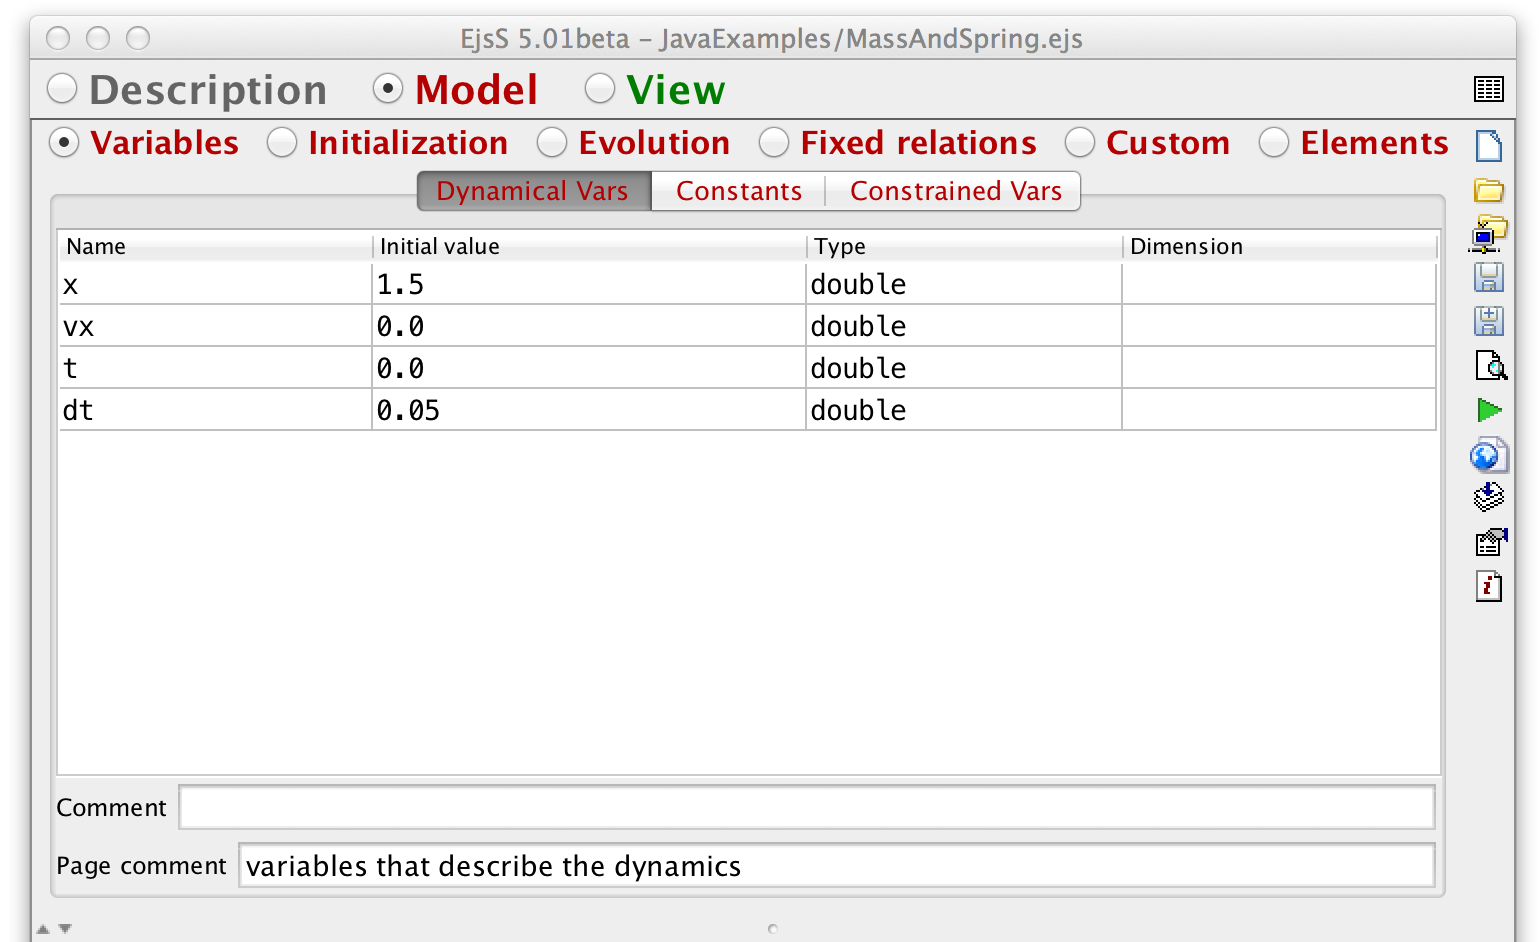
\includegraphics[scale=\scale]{02ExplorationJava/images/ModelVariables.png}
    \caption{The \lit{Model} workpanel contains six subpanels. The subpanel for the definition of mass and spring dynamical variables is displayed.  Other tabs in this subpanel define additional variables, such as the natural length of the spring $L$ and the energy $E$.} \label{fig:02ExplorationJava/ModelVariables}
\end{figure}

When implementing a model, a good first step is to identify, define, and initialize the variables that describe the
system. The term \emph{variable} is very general and refers to anything that can be given a name, including a
physical constant and a graph\index{Model!Variables}. Figure~\ref{fig:02ExplorationJava/ModelVariables} shows an
\ejs\ variable table. Each row defines a variable of the model by specifying the name of the variable, its type, its dimension, and its initial value.

Variables in computer programs can be of several types depending on the data they hold. The most frequently used types are \code{boolean} for true/false values, \code{int} for integers, \code{double} for high-precision ($\approx 16$ significant digits) numbers, and \code{String} for text.  We will use all these variable types in this document, but the mass and spring model uses only variables of type \code{double} and \code{boolean}.

Variables can be used as parameters, \index{Model!Parameters} state variables,\index{Model!State variables} or inputs and outputs of the model.\index{Model!Input and Output}  The tables in Figure~\ref{fig:02ExplorationJava/ModelVariables} define the variables used within our model.  We have
declared a variable for the $x$-position of the particle, \code{x}, for its velocity in the
$x$-direction, \code{vx}, for the time, \code{t}, and for the increment of time at each simulation step, \code{dt}.
We define some variables, in this and other tabs, that do not appear in Equation\eqref{eq:02ExplorationJava/SpringBasic}. The reason for auxiliary variables, such as  \code{vx} or the kinetic, potential, and total energies, will be made clear in what follows. The bottom part of the variables panel contains a comment field that provide a description of the role of each variable in the model. Clicking on a variable displays the corresponding comment.

\subsubsection{Initialization of the model}
Correctly setting initial conditions is important when implementing a model because the model must start in a
physically realizable state. Our model is relatively simple, and we initialize it by entering values (or simple Java
expressions such as \code{0.5*m*vx*vx}) in the \lit{Initial value} column of the table of variables. \ejs\ uses these values when it initializes the simulation.

\note{Advanced models may require an initialization algorithm. For example, a molecular dynamics model may set particle
velocities for an ensemble of particles. The \lit{Initialization} panel allows us to define one or more pages of Java
code that perform the required computation. \ejs\ converts this code into a Java method\index{Java!method}\footnote{A
Java method is similar to a function or a subroutine in procedural computer languages.} and calls this method at
start-up and whenever the simulation is reset. The mass and spring \lit{Initialization} panel is not shown here because
it is empty. See Subsection~\ref{section:02ExplorationJavaInspectingRelations} for an example of how Java code appears in \ejs.}

\subsubsection{The evolution of the model}

The \lit{Evolution} panel allows us to write the Java code that determines how the mass and spring system evolves in time and we will use this option frequently for models not based on ordinary differential equations (ODEs). There is, however, a second option that allows us to enter ordinary differential equations, such as \eqref{eq:02ExplorationJava/SpringBasic}, without programming.  \ejs\ provides a dedicated editor that lets us specify differential equations in a format that resembles mathematical
notation and automatically generates the correct Java code.

Let's see how the differential equation editor works for the mass and spring model. Because ODE algorithms solve
systems of first-order ordinary differential equations, a higher-order equation, such as
\eqref{eq:02ExplorationJava/SpringBasic}, must be recast into a first-order system.   We can do so by treating the
velocity as an independent variable which obeys its own equation:
\begin{align}
  \frac{d\ x} {dt} &= v_x                           \label{eq:02ExplorationJava/SpringBasicODE1} \\
  \frac{d\ v_x}{dt} &= -\frac{k}{m}\,(x-L). \label{eq:02ExplorationJava/SpringBasicODE2}
\end{align}
The need for an additional differential equation explains why we declared the \code{vx} variable in our table of
variables.

Clicking on the \lit{Evolution} panel displays the ODE editor shown in
Figure~\ref{fig:02ExplorationJava/ModelEvolution}.
\begin{figure}[htb]
    \centering
  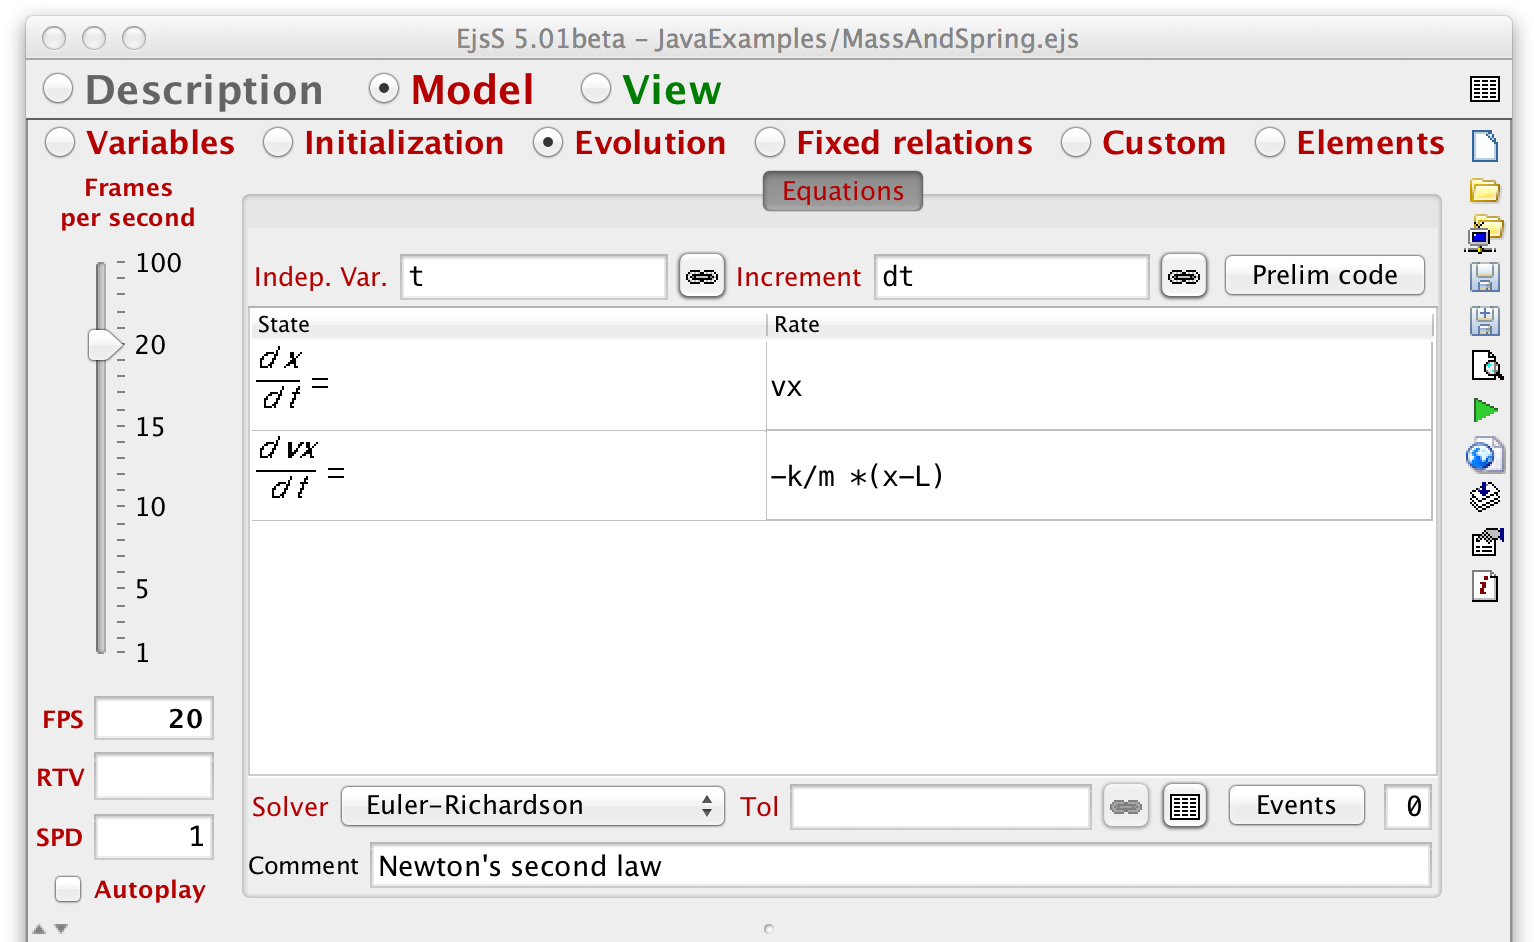
\includegraphics[scale=\scale]{02ExplorationJava/images/ModelEvolution.png}
    \caption{The ODE evolution panel showing the mass and spring differential equation and the numerical algorithm.}
    \label{fig:02ExplorationJava/ModelEvolution}
\end{figure}
Notice that the ODE editor displays \eqref{eq:02ExplorationJava/SpringBasicODE1} and \eqref{eq:02ExplorationJava/SpringBasicODE2}
(using the  \lit{*} character to denote multiplication). Fields near the top of the editor specify the independent variable
\code{t} and the variable increment \code{dt}.  Numerical algorithms approximate the exact ODE solution by advancing
the state in discrete steps and the increment determines this step size.
The \lit{Prelim code} button at the top-right of the editor allows us to enter preliminary code, to perform computations prior to evaluating the equations (a circumstance required in more complex situations than the one we treat in this example). A dropdown menu at the bottom of the editor
lets us select the ODE solver (numerical algorithm) that advances the solution from the current value of time, \code{t}, to the next value, \code{t + dt}. The tolerance field (\lit{Tol}) is greyed out and empty because Euler--Richardson is a fixed-step method that requires no tolerance settings. The advanced button displays a dialog which allows us to fine-tune the execution of this solver, though default values are usually appropriated. Finally, the events field at the bottom of the panel tells us that we have not defined any events for this differential equation. Examples with preliminary code and events can be found further on in this document. The different solver algorithms and its parameters are discussed in the \ejs\ help.

The left-hand side of the evolution workpanel includes fields that determine how smoothly and how fast the simulation runs.
The \lit{frames per second} (\lit{FPS}) option, which can be selected by using either a slider or an input field,
specifies how many times per second we want our simulation to repaint the screen. The \lit{steps per display}
(\lit{SPD}) input field specifies how many times we want to advance (step) the model before repainting. The current
value of \code{20} frames per second produces a smooth animation that, together with the prescribed value of one step
per display and \code{0.05} for \code{dt}, results in a simulation which runs  at (approximately) real time. We will
almost always use the default setting of one step per display. However, there are situations where the model's
graphical output consumes a significant amount of processing power and where we want to speed the numerical
computations. In this case we can increase the value of the steps per display parameter so that the model is advanced
multiple times before the visualization is redrawn. The \lit{Autoplay} check box indicates whether the simulation
should start when the program begins. This box is unchecked so that we can change the initial conditions before
starting the evolution.

The evolution workpanel handles the technical aspects of the mass and spring ODE model without programming.  The
simulation advances the state of the system by numerically solving the model's differential equations using the
midpoint algorithm. The algorithm steps from the current state at time \code{t} to a new state at a new time
\code{t + dt} before the visualization is redrawn. The simulation repeats this evolution step \code{20} times per second
on computers with modest processing power. The simulation may run slower and not as smoothly on computers with
insufficient processing power or if the computer is otherwise engaged, but it should not fail.

\note{Although the mass and spring model can be solved with a simple ODE algorithm, our numerical methods library
contains very sophisticated algorithms and \ejs\ can apply these algorithms to large systems of vector differential
equations with or without discontinuous events.}

\subsubsection{Relations among variables}\label{section:02ExplorationJavaInspectingRelations}
Not all variables within a model are computed using an algorithm on the Evolution workpanel. Variables can also be computed after the evolution has been applied. We refer to variables that are computed using the evolution algorithm as state variables or dynamical variables, and we refer to variables that depend on these variables as auxiliary or output variables. In the mass and
spring model the kinetic, potential, and total energies of the system are output variables because they are computed
from state variables.
\begin{align}
  T &= \frac{1}{2} m {v_x}^2,     \label{eq:02ExplorationJava/SpringEnergy1} \\
  V &= \frac{1}{2} k (x-L)^2,     \label{eq:02ExplorationJava/SpringEnergy2} \\
  E &= T + V.                     \label{eq:02ExplorationJava/SpringEnergy3}
\end{align}
We  say that there exists \emph{fixed relations} among the model's variables.

The \lit{Fixed relations} panel shown in Figure~\ref{fig:02ExplorationJava/ModelRelations} is used to write relations among
variables. Notice how easy it is to convert \eqref{eq:02ExplorationJava/SpringEnergy1} through
\eqref{eq:02ExplorationJava/SpringEnergy3} into Java syntax. Be sure to
use the multiplication character \lit{*} and to place a semicolon at the end of each Java statement.

\begin{figure}[htb]
    \centering
  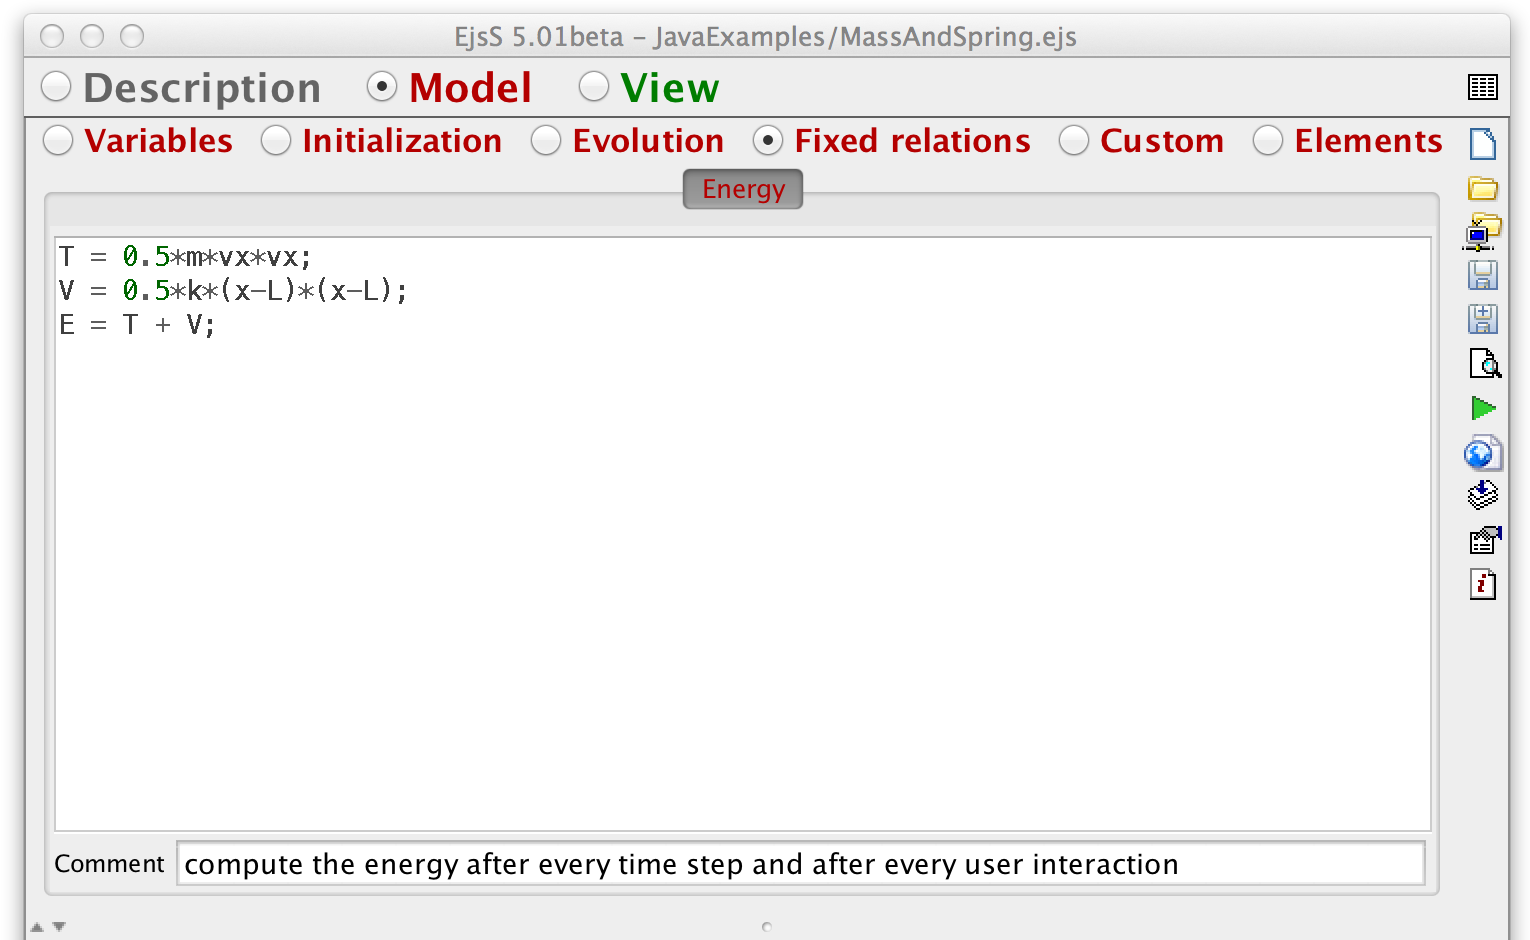
\includegraphics[scale=\scale]{02ExplorationJava/images/ModelConstraints.png}
    \caption{Fixed relations for the mass and spring model.}
    \label{fig:02ExplorationJava/ModelRelations}
\end{figure}

\noindent \textbf{Here goes an important remark.} You may wonder why we do not write fixed relation expressions by adding a second code page after the ODE page in the
\lit{Evolution} panel. After all, evolution pages execute sequentially and a second evolution page would correctly
update the output variables after every step. The reason that the \lit{Evolution} panel should not be used is that
relations must \emph{always} hold and there are other ways, such as mouse actions, to affect state
variables. For example, dragging the mass changes the $x$ variable and this change affects the energy.
\ejs\ automatically evaluates the relations after initialization, after every evolution step, and whenever
there is any user interaction with the simulation's interface.  For this reason, it is important that fixed relations among variables be written in the \lit{Fixed relations} workpanel.

\subsubsection{Custom pages}

There is a fifth panel in the \lit{Model} workpanel labeled \lit{Custom}. This panel can be used to define Java methods (functions) that can be used throughout the model.  This panel is empty because our model currently doesn't require additional methods,
but we will make use of this panel when we modify our mass and spring example in Section~\ref{section:02ExplorationJavaModifying}.  A
custom method is not used unless it is explicitly invoked from another workpanel.

\subsubsection{Model elements}

The final, sixth panel in the \lit{Model} workpanel is labeled \lit{Elements} and provides access to third-party Java libraries in the form of drag and drop icons. You add these libraries to your program by dragging the corresponding icon to the list of model elements to use for this model. This creates Java objects you can then use in your model code. This panel is also empty for this model because our mass and spring doesn't require additional Java libraries.

% ---------------------------------------------
\subsection{The \lit{View} workpanel}
% ---------------------------------------------

The third \Ejs\ workpanel is the \lit{View}.  This workpanel allows us to create a graphical interface that includes
visualization, user interaction, and program control with minimum programming.
Figure~\ref{fig:02ExplorationJava/SpringInterface} shows the view for the mass and spring model. Select the \lit{View} radio
button to examine how this view is created.

The right frame of the view workpanel of \ejs, shown in Figure~\ref{fig:02ExplorationJava/View}, contains a collection of
\emph{view elements},\index{Ejs!view elements} grouped by functionality. View elements are building blocks that can be
combined to form a complete user interface, and each view element is a specialized object with an on-screen
representation. To display information about a given element, click on its icon and press the \lit{F1} key or right-click and select the \lit{Help} menu item. To create a user interface, we create a frame (window) and add elements, such as buttons and graphs, using ``drag and drop'' as described in Section~\ref{section:02ExplorationJavaModifying}.

\begin{figure}[htb]
    \centering
  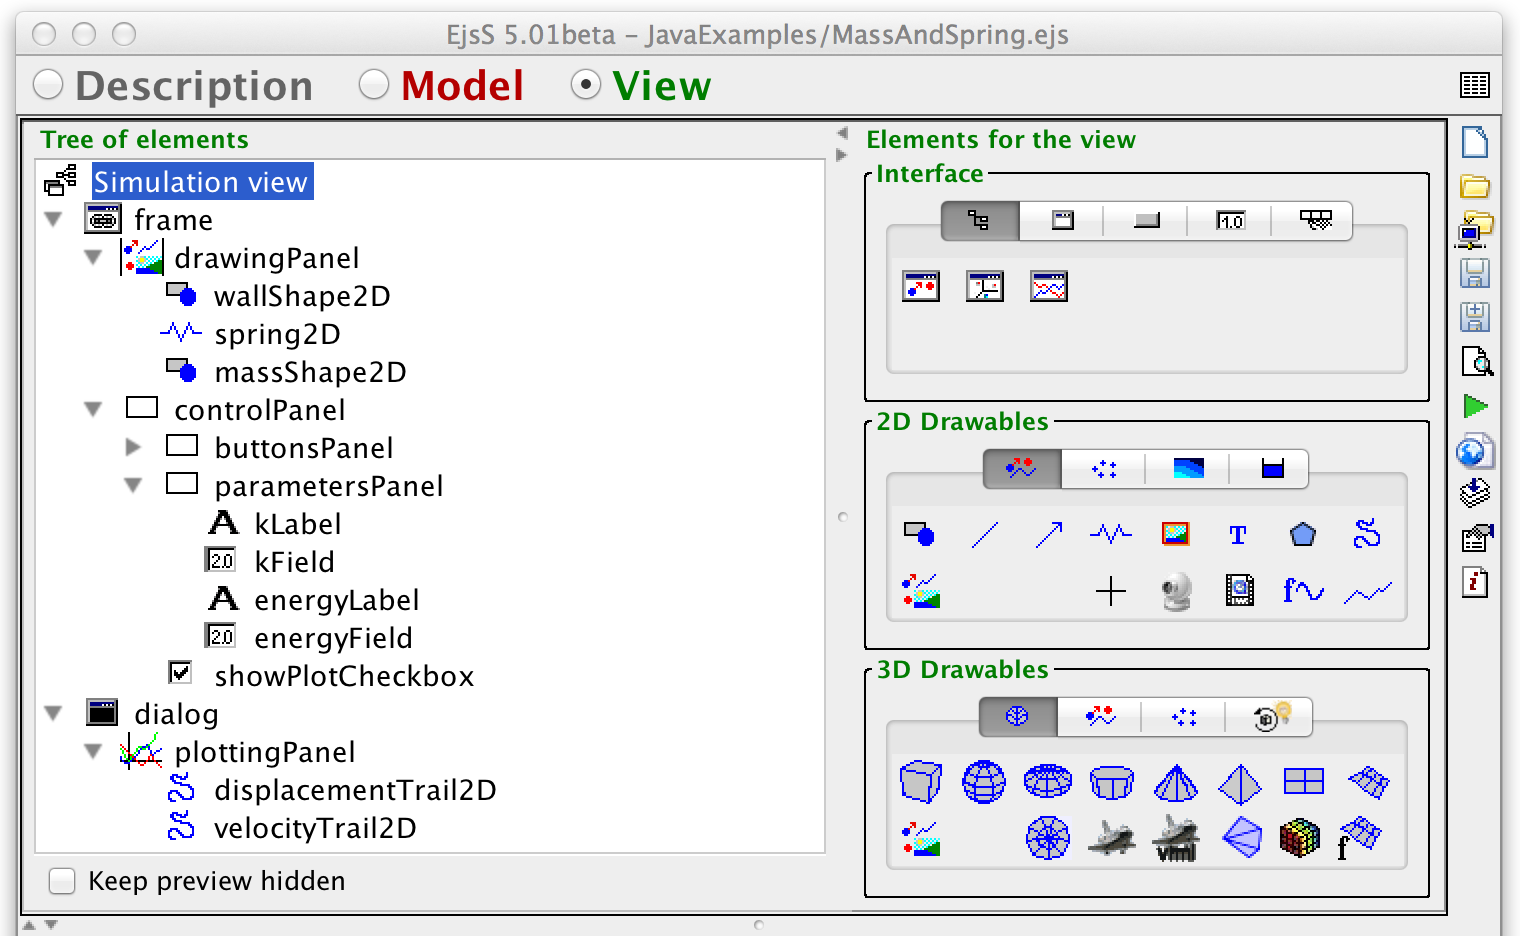
\includegraphics[scale=\scale]{02ExplorationJava/images/View.png}
    \caption{The \lit{View} workpanel showing the \emph{Tree of elements} for the mass and spring user interface.}
    \label{fig:02ExplorationJava/View}
\end{figure}

The \emph{Tree of elements} shown on the left side of Figure~\ref{fig:02ExplorationJava/View} displays the structure of the
mass and spring user interface. Notice that the simulation has two windows, a \code{Frame} and a \code{Dialog}, that appear on your computer screen.
These elements belong to the class of \emph{container} elements whose primary
purpose is to visually group (organize) other elements within the user interface.
The tree displays descriptive names and icons for these elements.   Right-click on an element of the tree to
obtain a menu that helps the user change this structure. Alternatively, you can drag and drop elements from one container to another to change the parent-child relationship, or within a container to change the child order. (There are conditions for a container to accept a given element as child. For instance, a two-dimensional drawing panel can only accept 2D drawable elements.)

Each view element has a set of internal parameters, called \emph{properties},\index{Ejs!view element properties} which
configure the element's appearance and behavior. We can edit these properties by double clicking on the element in the
tree to display a table known as a \emph{properties inspector}.  Appearance properties, such as color, are often set to a constant value, such as \code{RED}. We can also use a variable from the model to set an element's property. This ability to connect (bind) a property to a variable without programming is the key to turning our view into a dynamic and interactive
visualization.

Let's see how this procedure works in practice. Double-click on the \code{massShape2D} element (the `Shape2D' suffix we added to the element's name helps you know the type of the element) in the tree to display
the element's properties inspector. This element is the mass that is attached at the free end of the spring. The massShape2D's table of properties appears as shown in Figure~\ref{fig:02ExplorationJava/SpringBallProperties}.
\begin{figure}[htb]
    \centering
  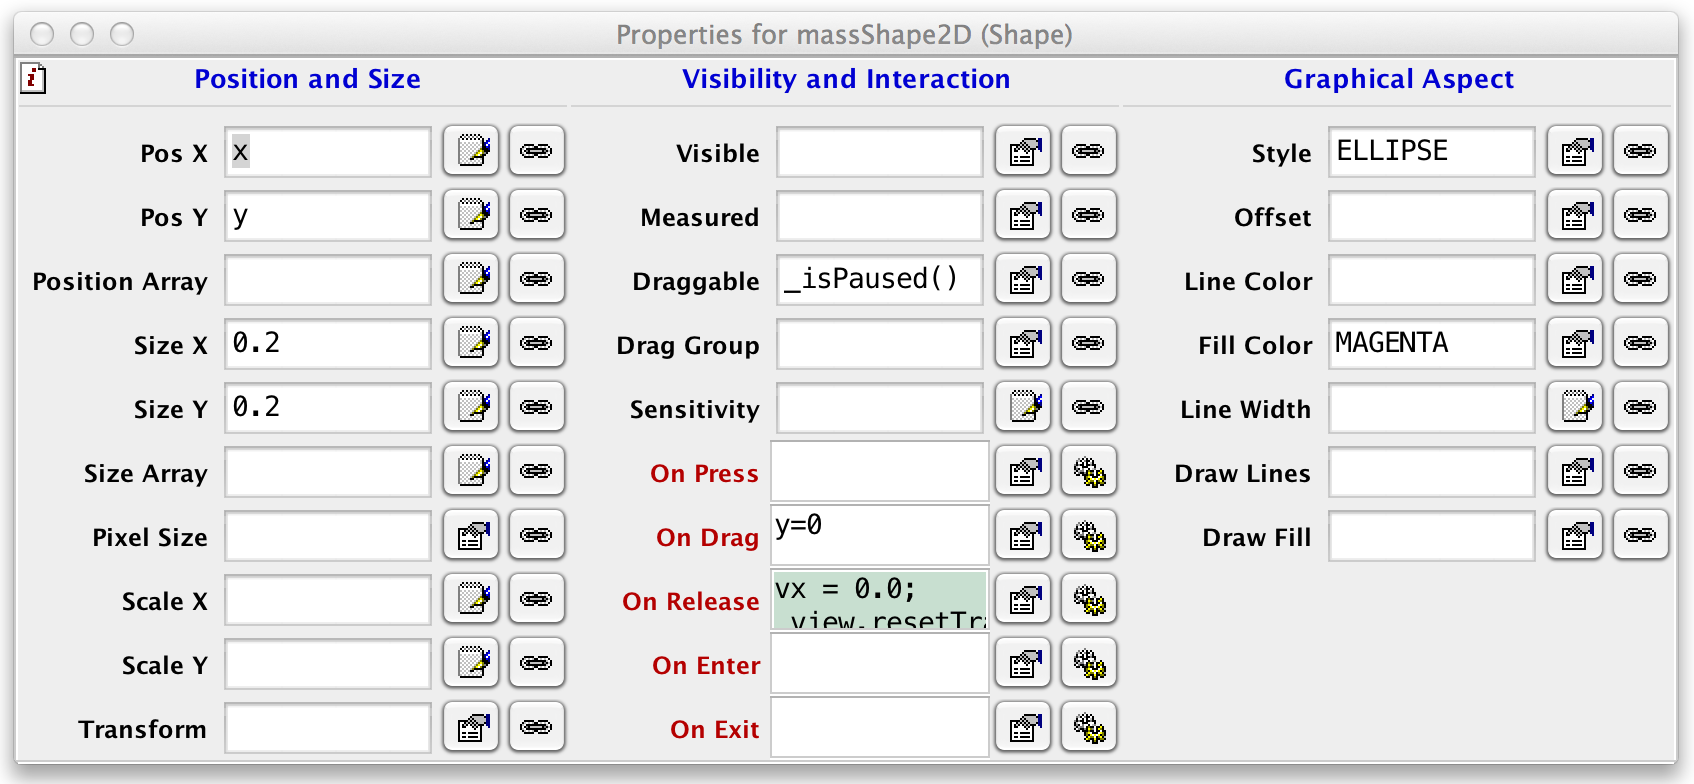
\includegraphics[scale=\scale]{02ExplorationJava/images/SpringBallProperties.png}
    \caption{The table of properties of the \code{massShape2D} element.}
    \label{fig:02ExplorationJava/SpringBallProperties}
\end{figure}

Notice the properties that are given constant values. The \code{Style}, \code{Size X}, \code{Size Y}, and \code{Fill
Color} properties produce an ellipse of size \code{(0.2,0.2)} units (which makes a circle) filled with the color
magenta. More importantly, the \code{Pos X} and \code{Pos Y} properties of  the shape are bound to the \code{x} and \code{y}
variables of the model. This simple assignment establishes a bidirectional connection between model and view. These
variables change as the model evolves and the shape follows the \code{x} and \code{y} values. If the user drags the
shape to a new location, the \code{x} and \code{y} variables in the model change accordingly.  Note that the \code{Draggable} property is only enabled when the animation is paused.

Elements can also have \emph{action properties}\index{Ejs!action properties} which can be associated with code.
(Action properties have their labels displayed in red.) User actions, such as dragging or clicking, invoke their
corresponding action property, thus providing a simple way to control the simulation. As the user drags the mass, the code on the \code{On Drag} property restricts the motion of the shape to the horizontal direction by setting the \code{y} variable to \code{0}.  Finally, when the mouse button is
released, the following code is executed:

\begin{listing}
\begin{verbatim}
vx = 0.0;            // sets the velocity to zero
_view.resetTraces(); // clears all plots
\end{verbatim}
\end{listing}

\noindent Clicking on the icon next to the field displays a small editor that shows this code.

\note{Because the \code{On Release} action code spans more than one line, the property field in the inspector shows a darker (green) background. Other data types, such as boolean properties, have different editors.  Clicking the second icon displays a dialog window with a listing of variables and methods that can be used to set the property value.}

\begin{exercise}[Element inspectors]\label{ex:02ExplorationJava/properties}
The mass' inspector displays different types of properties and their possible values. Explore the properties of other
elements of the view.  For instance, the \code{displacementTrail2D} and \code{velocityTrail2D} elements correspond to the
displacement and velocity time plots in the second window of the view, respectively.  What is the maximum number of points that can be added to each trail?
\end{exercise}

\subsection{The completed simulation}

We have seen that \Ejs\ is a powerful tool that lets us express our knowledge of a model at a very high level of abstraction. When modeling the mass and spring, we first created a table of variables that describes the model and initialized these variables using a column in the table. We then used an evolution panel with a high-level editor for systems of first-order ordinary differential equations to specify how the state advances in time. We then wrote relations to compute the auxiliary or output variables that can be expressed using expressions involving state variables.  Finally, the program's graphical user interface and high-level visualizations were created by dragging objects from the \lit{Elements} palette into the \lit{Tree of elements}. Element properties were set using a properties editor and some properties were associated with variables from the model.

It is important to note that the three lines of  code on the Fixed relations workpanel (Figure~\ref{fig:02ExplorationJava/ModelRelations}) and the two lines of code in the particle's action method are the only explicit Java code needed to implement the model.  \Ejs\ creates a complete Java program by processing the information in the workpanels when the run icon is pressed as described in Section~\ref{section:02ExplorationJavaRunning}.

% -----------------------------------------------------
\section{Running the Simulation}\label{section:02ExplorationJavaRunning}\index{Simulation!running}
% -----------------------------------------------------

It is time to run the simulation by clicking on the \lit{Run} icon of the taskbar, 
\includegraphics[scale=\linescale]{../_common/icons_png/launch.png}.  \ejs\ generates the Java code and compiles it, collects auxiliary and library files, and executes the compiled program. All at a single mouse click.

Running a simulation initializes its variables and executes the fixed relations to insure that the model is in a consistent state.  The model's time evolution starts when the play/pause button in the user interface is pressed. (The play/pause button displays the 
\includegraphics[scale=\linescale]{../_common/icons_png/play.png} icon when the simulation is paused and 
\includegraphics[scale=\linescale]{../_common/icons_png/pause.png} when it is running.) In our current example, the program executes a numerical method to advance the harmonic oscillator differential equation by $0.05$ time units and then executes the fixed relations code.  Data are then passed to the graph and the graph is repainted. This process is repeated $20$ times per second.

When running a simulation, \ejs\ changes its \lit{Run} triangle icon to a red \lit{Kill} square and prints informational messages saying that the
simulation has been successfully generated and that it is running. Notice that the two \ejs\ windows disappear and are
replaced by new but similar windows without the \code(Ejs window) suffix in their titles.  These views respond to user
actions. Click and drag the particle to a desired initial horizontal position and then click on the play/pause button.
The particle oscillates about is equilibrium point and the plot displays the displacement and velocity data as shown in
Figure~\ref{fig:02ExplorationJava/SpringRunning}.

Stop the simulation and right-click the mouse over any of the drawing areas of the simulation. In the popup menu that appears, select the \code{Elements options->plottingPanel->Data Tool} entry to display and analyze the data generated by the model.  The same popup menu offers other run-time options, such as screen capture.  To exit the program, close the simulation's main window.

\begin{figure}[htb]
  \centering
  \subfigure{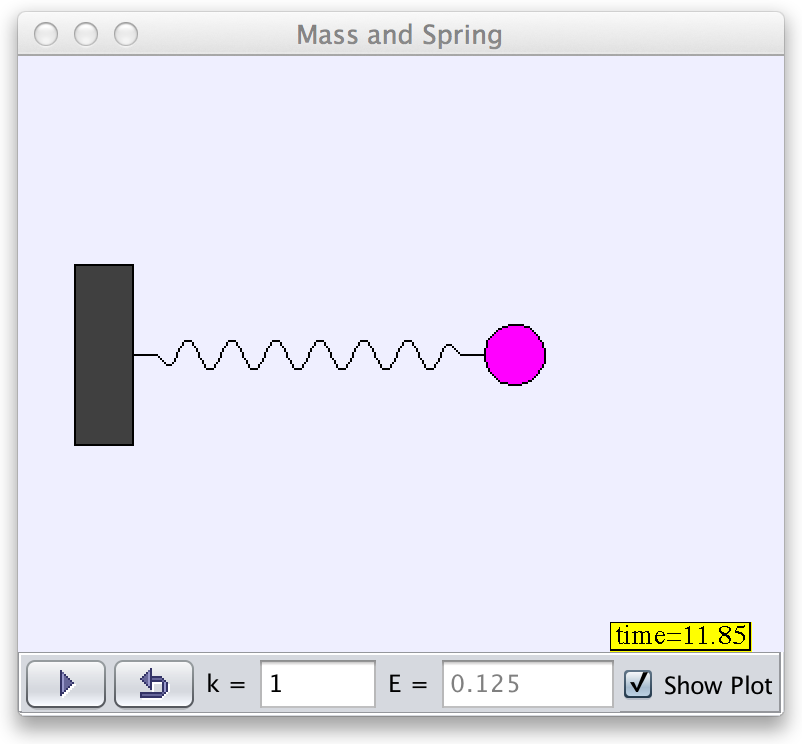
\includegraphics[scale=\scale]{02ExplorationJava/images/SpringRunning1.png}}
  \subfigure{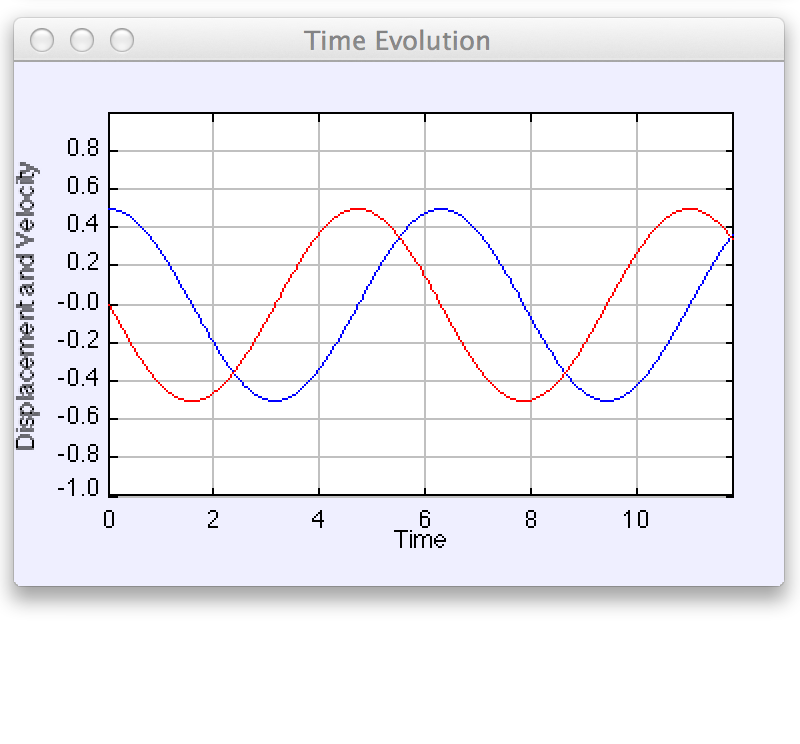
\includegraphics[scale=\scale]{02ExplorationJava/images/SpringRunning2.png}}
  \caption{The mass and spring simulation displays an interactive drawing of the model and a graph with displacement and velocity data.}
  \label{fig:02ExplorationJava/SpringRunning}
\end{figure}


% -----------------------------------------------------
\section{Distributing the Simulation}\label{section:02ExplorationJavaDistributing}\index{Simulation!distribution}
%
Simulations created with \ejs\ are stand-alone Java programs that can be distributed without \ejs\ for other people to use.  The easiest way to do this is to package the simulation in a single executable jar file by clicking on the \lit{Package} icon, 
\includegraphics[scale=\linescale]{../_common/icons_png/package.png}. A file browser appears that lets you choose a name for the self-contained jar package.  The default target directory to hold this package file is the \file{export} directory of your workspace, but you can choose any directory and package name. The stand-alone jar file is ready to be distributed on a CD or via the Internet.  Other distribution mechanisms are available by right-clicking on the icon.
% as described in Appendix~\ref{appendix:Distribution}.

\begin{exercise}[Distribution of a model]\label{ex:02ExplorationJava/distribution}
Click on the \lit{Package} icon on the taskbar to create a stand alone jar archive of the mass and spring simulation.  Copy this jar file into a working directory separate from your \ejs\ installation.  Close \ejs\ and verify that the simulation runs as a stand-alone application.
\end{exercise}

Although the mass and spring jar file is a ready to use and to distribute Java application, an important pedagogic feature is that this jar file is created in such a way that users can return to \ejs\ at any time to examine, modify, and adapt the model. (\ejs\ must, of course, be installed.)  The jar file contains a small \emph{Extensible Markup Language} (XML) description of each model and right clicking on a drawing panel within the model brings in a popup menu with an option to copy this file into \ejs. This action will extract the required files from the jar, search for the \ejs\ installation in the user's hard disk, copy the files into the correct location, and run \ejs\ with this simulation loaded. If a model with the same name already exits, it can be replaced. The user can then inspect, run, and modify the model just as we are doing in this chapter.  A student can, for example, obtain an example or a template from an instructor and can later repackage the modified model into a new jar file for submission as a completed exercise.

\begin{exercise}[Extracting a model]\label{ex:02ExplorationJava/redistribution}
Run the stand-alone jar file containing the mass and spring model created in Exercise~\ref{ex:02ExplorationJava/distribution}.  Right click on the model's plot or drawing and select the \lit{Open Ejs Model} item from the popup menu to copy the packaged model back into \ejs.
\end{exercise}

\ejs\ is designed to be both a modeling and an authoring tool, and we suggest that you now experiment with it to learn
how you can create and distribute your own models. As a start, we recommend that you run the mass and spring simulation
and go through the activities in the second page of the \lit{Description} workpanel.  We modify this simulation in the next
section.

% -----------------------------------------------------
\section{Modifying the Simulation}\label{section:02ExplorationJavaModifying}
% -----------------------------------------------------

As we have seen, a prominent and distinctive feature of \Ejs\ is that it allows us to create and study a simulation at
a high level of abstraction. We inspected an existing mass and spring model and its user interface in the previous
section. We now illustrate additional capabilities of \Ejs\ by adding friction and a driving force and by adding a
visualization of the system's phase space.

\subsection{Extending the model}\label{section:02ExplorationJavaModifyingModel}
We can add damping in our model by introducing a viscous (Stoke's law) force that is proportional to the negative of
the velocity $F_f = - b\,v_x$ where $b$ is the damping coefficient. We also add an external time-dependent driving
force which takes the form of a sinusoidal function $F_e(t)=A\,\sin(\omega\, t)$. The introduction of these two forces
changes the second-order differential equation \eqref{eq:02ExplorationJava/SpringBasic} to
\begin{equation}
  \frac{d^2\ x}{dt^2} = -\frac{k}{m}\,(x-L) - \frac{b}{m}\,\frac{d\ x}{dt} + \frac{1}{m}\,F_e(t), \label{eq:02ExplorationJava/SpringComplete}
\end{equation}
or, as in equations \eqref{eq:02ExplorationJava/SpringBasicODE1} and \eqref{eq:02ExplorationJava/SpringBasicODE2}:
\begin{eqnarray}
  \frac{d\ x} {dt} &=& v_x,                  \label{eq:02ExplorationJava/SpringCompleteODE1} \\
  \frac{d\ v_x}{dt} &=& -\frac{k}{m}\,(x-L) - \frac{b}{m}\,v_x + \frac{1}{m}\,F_e(t). \label{eq:02ExplorationJava/SpringCompleteODE2}
\end{eqnarray}

\subsubsection{Adding variables}
The introduction of new force terms requires that we add variables for the coefficient of dynamic friction and for the amplitude and frequency of the sinusoidal driving force.  Return to the \lit{Model} workpanel of \ejs\ and select its \lit{Variables} panel. Right-click on the tab of the existing page of variables to see its popup menu, as in Figure~\ref{fig:02ExplorationJava/ModifyVariables1}.
Select the \lit{Add a new page} entry as shown in Figure~\ref{fig:02ExplorationJava/ModifyVariables1}. Enter \code{Damping and Driving Vars} for the new table name in the dialog and an empty table will appear.

\begin{figure}[htb]
    \centering
  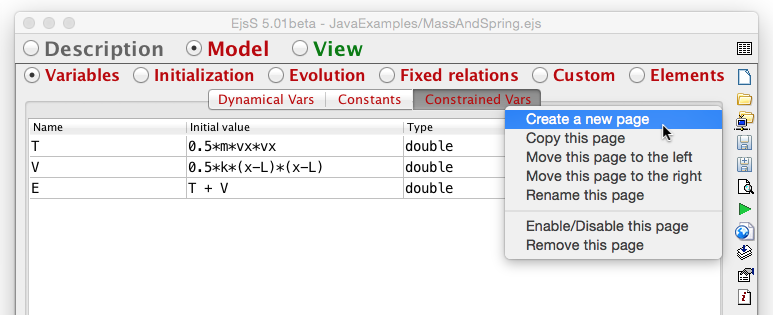
\includegraphics[scale=\scale]{02ExplorationJava/images/ModifyVariables1.png}
    \caption{The popup menu for a page of variables.}
    \label{fig:02ExplorationJava/ModifyVariables1}
\end{figure}

We now use the new table to declare the needed variables. We could have used the already existing tables, but declaring multiple pages helps us organize the variables by category. Double-click on a table cell to make it editable and navigate through the table using the arrows or tab keys. Type \code{b} in the \lit{Name} cell of the first row, and enter the value \code{0.1} in the \lit{Initial value} cell to its right. We don't need to do anything else because the \code{double} type selected is already correct.
\ejs\ checks the syntax of the value entered and evaluates it. If we enter a wrong value, the background of the value cell will display a pink background.
Notice that when you fill in a variable name, a new row appears automatically. Proceed similarly to declare a new variable for the driving force's \code{amp} with value \code{0.2} and for its \code{freq} with value \code{2.0}. Document the meaning of these variables by typing a short comment for each at the bottom of the table. Our final table of variables is shown in Figure~\ref{fig:02ExplorationJava/ModifyVariables2}.  You can ignore the empty row at the end of the table or remove it by right-clicking on that row and selecting \lit{Delete} from the popup menu that appears.

\begin{figure}[htb]
    \centering
  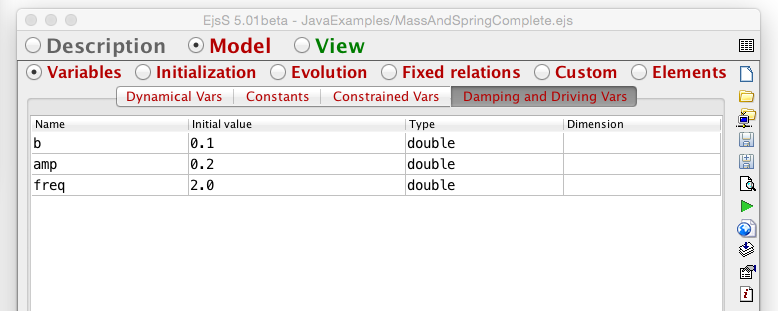
\includegraphics[scale=\scale]{02ExplorationJava/images/ModifyVariables2.png}
    \caption{The new table of variables for the damping and forcing terms.}
    \label{fig:02ExplorationJava/ModifyVariables2}
\end{figure}

\subsubsection{Modifying the evolution}

We now modify the differential equations on the evolution page by adding expressions for the new terms in equation
\eqref{eq:02ExplorationJava/SpringCompleteODE2}. Go to the evolution panel, double-click on the \lit{Rate} cell of the
second equation, and edit it to read:

\begin{listing}
\begin{verbatim}
-k/m * (x-L) - b*vx/m + force(t)/m
\end{verbatim}
\end{listing}
Notice that we are using a method (function) named \code{force} that has not yet been defined.
We could have written an explicit expression for the sinusoidal function. However, defining a \code{force} method promotes cleaner and more readable code and allows us to introduce custom methods.

\subsubsection{Adding custom code}

The \code{force} method is defined using the \lit{Custom} panel of the \lit{Model}. Go to this panel and click on the
empty central area to create a new page of custom code. Name this page \lit{force}. You will notice that the
page is created with a code template that defines the method. Edit this code to read:

\begin{listing}
\begin{verbatim}
public double force (double time) {
  return amp*Math.sin(freq*time); // sinusoidal driving force
}
\end{verbatim}
\end{listing}
Type this code exactly as shown including capitalization. Compilers complain if there is any syntax error.

Notice that we pass the time at which we want to compute the driving force to the \texttt{force} method as an input parameter. Passing
the time value is very important. It would be incorrect to ask the method to use the value of the variable \code{t}, as
in:

\begin{listing}
\begin{verbatim}
public double force () { // incorrect implementation of the force method
  return amp*Math.sin(freq*t);
}
\end{verbatim}
\end{listing}

\noindent The reason that time must be passed to the method is that time changes throughout the evolution step.  In order for the ODE solver to correctly compute the time-dependent force throughout the evolution step, the time must be passed into the method that computes the rate.

\note{ Variables that change (evolve) must be passed to methods that are used to compute the rate because numerical solvers evaluate the \lit{Rate} column in the ODE workpanel at intermediate values between $t$ and $t+dt$. In other words, the independent variable and any other dynamic variable which is differentiated in the \lit{State} column of the ODE editor must be passed to any method that is called in the \lit{Rate} column. Variables which remain constant during an evolution step may be used without being passed as input parameters because the value of the variable at the beginning of the evolution step can be used.}

\subsection{Improving the view}\label{section:02ExplorationJavaModifyingView}
We now add a visualization of the phase space (displacement versus velocity) of the system's evolution to the
\lit{View}. We also add new input fields to display and modify the value of the damping, amplitude, and frequency parameters.

Go to the \lit{View} workpanel and notice that the \lit{Interface} palette contains many subpanels.  Click on the tab
with the 
\includegraphics[scale=\linescale]{../_common/icons_png/Groups/Containers.png} icon to display the \lit{Windows, containers,
and drawing panels} palette of view elements.  Click on the icon for a plotting panel,

\includegraphics[scale=\linescale]{../_common/icons_png/Elements/PlottingPanel.png}, in this palette. You can rest (hover) the mouse
cursor over an icon to display a hint that describes the element if you have difficulty recognizing the icon.
Selecting an element sets a colored border around its icon on the palette and changes the cursor to a magic wand,

\includegraphics[scale=\linescale]{../_common/icons_png/create.png}. These changes indicate that \ejs\ is ready to create
an element of the selected type. (Return to the design mode --get rid of the magic wand-- by clicking on any
blank area within the \lit{Tree of elements} or hitting the \lit{Esc} key.)

Click on the \code{dialog} element in the \lit{Tree of elements} as shown in
Figure~\ref{fig:02ExplorationJava/ModifyViewAddPlottingPanel} to add the plotting panel to the view.

\begin{figure}[htb]
    \centering
  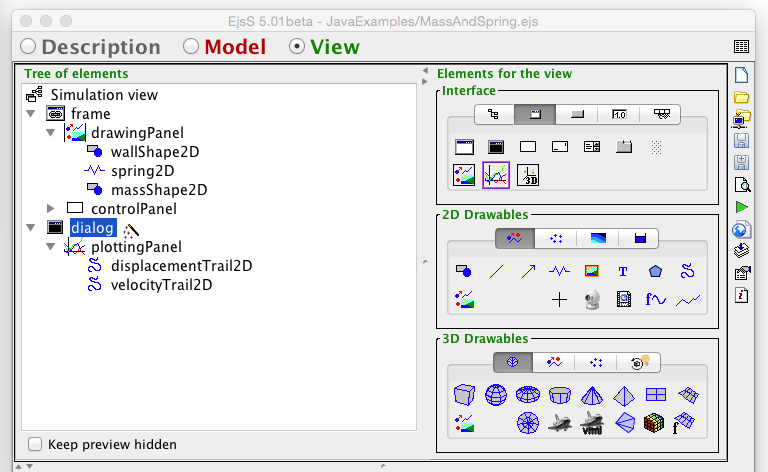
\includegraphics[scale=\scale]{02ExplorationJava/images/ModifyViewAddPlottingPanel.png}
    \caption{Creation of a plotting panel as a child of the \code{dialog} element of the view.}
    \label{fig:02ExplorationJava/ModifyViewAddPlottingPanel}
\end{figure}

\ejs\ asks for the name of the new element and then creates the element as a child within the existing \code{dialog}. A
new plot appears but the dialog is too small.  Resize the dialog box by dragging its
corner. You can also resize the dialog box by double-clicking on the \code{dialog} element in the tree to show its
properties table and changing its \code{Size} property to \code{"385,524"}, thus doubling its height. Finally, edit the
properties table of the newly created plotting panel element to set the \code{Title} property to \code{Phase Space},
the \code{Title X} property to \code{Displacement}, and the \code{Title Y} property to \code{Velocity}. (\ejs\ will
add leading and trailing quotes to these strings to conform to the correct Java syntax.) Set the minima
and maxima for both X and Y scales to \code{-1} and {1}, respectively, and leave the other properties untouched.

The plotting panel is, as its name suggests, the container for the phase-space plot. Phase space data are drawn in this
panel using an element of type \code{Trail2D}, 
\includegraphics[scale=\linescale]{../_common/icons_png/Elements/Trail.png}.  Find the
\code{Trail2D} element in the \code{2D Drawables} palette and follow the same procedure as before.  Select the
\code{Trail2D} element and create an element of this type by clicking with the magic wand on the phase space panel.
Finally, edit the properties of the new trail element to set its \code{Input X} property to \code{x - L} and its
\code{Input Y} property to \code{vx}. This assignment causes the simulation to add a new \code{(x - L,vx)} point to the
trace after each evolution step, thus drawing the phase-space plot shown in Figure~\ref{fig:02ExplorationJava/ModifyRunning}.

\begin{figure}[htb]
  \centering
  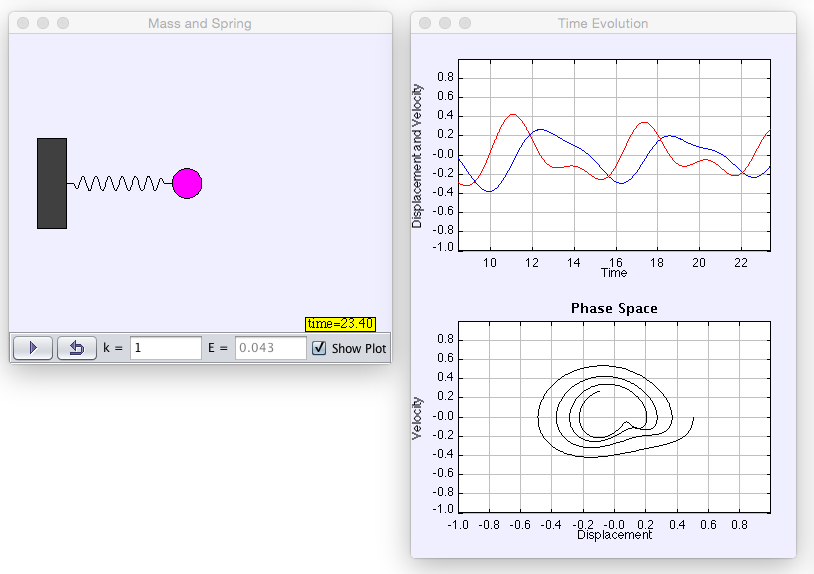
\includegraphics[scale=\scale]{02ExplorationJava/images/ModifyRunning.png}
  \caption{The modified simulation. The dialog includes now both a time and a phase-space plot.}
  \label{fig:02ExplorationJava/ModifyRunning}
\end{figure}

To finish the modifications, we add a new panel to the top of the drawing frame that shows the sinusoidal driving force parameters.

\begin{bulletlist}

\item Select the \code{Panel} element icon, 
\includegraphics[scale=\linescale]{../_common/icons_png/Elements/Panel.png}, on the \lit{Windows, containers, and drawing panels} subgroup of the \lit{Interface} palette. Click with the magic wand on the element named \code{frame} within the \lit{Tree of elements} to create a new panel named \code{forceParamPanel} in the frame's top location. Use the properties inspector to set this panel's layout to \lit{FLOW:center,0,0} and its border type to \texttt{LOWERED\_ETCHED}.
\item Select the \code{Label} element icon, 
\includegraphics[scale=\linescale]{../_common/icons_png/Elements/Label.png}, on the \lit{Buttons and decorations} subgroup of the \lit{Interface} palette and create a new element of that type in the \code{forceParamPanel} panel.  Set the label's text property to \texttt{"frequency ="}.
\item Select the \code{Field} element icon, 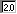
\includegraphics[scale=\linescale]{../_common/icons_png/Elements/ParsedField.png}, and create a new element named \code{freqField} in the force parameter panel.  Edit the \code{freqField} properties table as shown in Figure~\ref{fig:02ExplorationJava/ModifyField}. The connection to the \code{freq} variable is established using the \code{Variable} property.  Click on the second icon to the right of the property field, 
\includegraphics[scale=\linescale]{../_common/icons_png/link.png}, and choose the appropriate variable. The variable list shows all the model variables that can be used to set the property field. The \code{Format} property indicates the number of decimal digits with which to display the value of the variable.
\item Repeat this process to add the \code{amp} variable to the user interface.
\end{bulletlist}

\begin{figure}[htb]
    \centering
  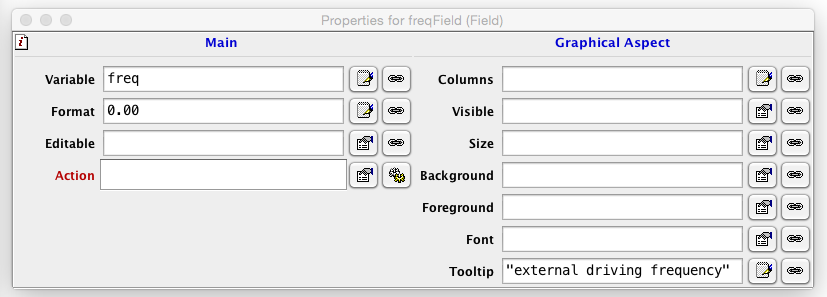
\includegraphics[scale=\scale]{02ExplorationJava/images/ModifyField.png}
    \caption{The table of properties of the \code{freqField} element.}
    \label{fig:02ExplorationJava/ModifyField}
\end{figure}

\subsection{Changing the description}\label{section:02ExplorationJavaModifyingDescription}

Now that we have changed the model and the view, we should modify the description pages of our simulation. Go to the \lit{Description} workpanel and click on the tab of the first page, the one labeled \code{Introduction}. Once you see this page, click the \lit{Click to modify the page} icon, 
\includegraphics[scale=\linescale]{../_common/icons_png/edit.png}. The description page will change to edit mode, as shown in Figure~\ref{fig:02ExplorationJava/ModifyHTML}, and a simple editor will appear that provides direct access to common HTML features.

If you prefer to use your own editor, you can copy and paste HTML fragments from your editor into the \ejs\ editor. If you know HTML syntax, you can enter tagged (markup) text directly by clicking the source icon, 
\includegraphics[scale=\linescale]{02ExplorationJava/images/SourceHK.png}, in the tool bar.  You can even import entire HTML pages into \ejs\ by clicking the \lit{Link/Unlink page to external file} icons, 
\includegraphics[scale=\linescale]{../_common/icons_png/link.png}, 
\includegraphics[scale=\linescale]{../_common/icons_png/unlinked.png}.

\begin{figure}[htb]
    \centering
  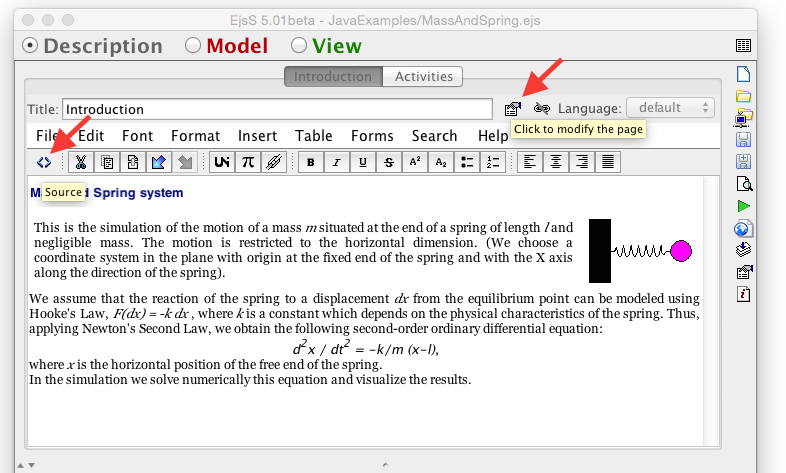
\includegraphics[scale=\scale]{02ExplorationJava/images/ModifyHTML.png}
    \caption{The HTML editor of \ejs. The added red arrows point to the edit and source code edition mode icons.}
    \label{fig:02ExplorationJava/ModifyHTML}
\end{figure}

Edit the description pages as you find convenient. At least change the discussion of the model to include the damping and driving forces. When you are done, save the new simulation with a different name by clicking the \lit{Save as} icon of \ejs' taskbar, 
\includegraphics[scale=\linescale]{../_common/icons_png/saveAsSmall.png}. When prompted, enter a new name for your simulation's XML file. The modified simulation is stored in the \file{MassAndSpringComplete.ejs} file in the \file{source} directory for this chapter.

% -----------------------------------------------------
\section{Problems and Projects}\label{section:02ExplorationJavaProjects}
% -----------------------------------------------------

%\subsection*{Problem 1}
\begin{problem}[Energy]
Add a third plotting panel to the dialog window of the \file{MassAndSpringComplete.ejs} simulation that will display the evolution of the kinetic, potential, and total energies.
\end{problem}

%\subsection*{Problem 2}
\begin{problem}[Function plotter]
The analytic solution for the undriven simple harmonic oscillator is
\begin{equation}
  x(t)=A \sin(w_0 t + \phi)
\end{equation}
where $A$ is the amplitude (maximum displacement), $w_0= \sqrt{k/m}$ is the natural frequency of oscillation, and
$\phi$ is the phase angle.  Consult a mechanics textbook to determine the relationship between the amplitude and phase
angle and the initial displacement and velocity.  Use the \file{FunctionPlotter.ejs} simulation in the
examples directory to compare the analytic solution to the numerical solution generated by the
\file{MassAndSpringComplete.ejs} model.
\end{problem}

%\subsection*{Project 2}
\begin{project}[Two-dimensional oscillator]
Modify the model of the mass and spring simulation to consider motion that is not restricted to the horizontal
direction.  Assume that a second spring with spring constant $k'$ produces a vertical restoring force $F_y(\delta y) = - k' \,\delta y$. Modify the simulation to allow the user to specify the Hooke's law constants as well as the initial conditions in both directions. Describe the motion produced without a driving force but under different initial conditions and with different spring constants. (Try $k=1$ and $k'=9$.)  Show that it is possible to obtain circular motion if $k=k'$.
\end{project}

%\subsection*{Project 3}
\begin{project}[Simple pendulum]
Create a similar simulation as the one described in this chapter for a simple pendulum whose second-order differential
equation of motion is
\begin{equation}
  \frac{d^2\theta}{dt^2} = -\frac{g}{L} \sin (\theta),
\end{equation}
where $\theta$ is the angle of the pendulum with the vertical, $g$ is the acceleration due to gravity, and $L$ is the arms's length. Use fixed relations to compute the $x$ and $y$ position of the pendulum bob using the equations:
\begin{align*}
   x   &=  L \, \sin (\theta) \\
   y   &= -L \, \cos (\theta).
\end{align*}
\end{project}
